% F087｜牛顿切线法快速求近似根｜06_summary.tex
% 继承上传模板的 LaTeX 环境；当前条目的内容独立编写。
\clearpage
\begin{summarybox}
\textbf{\textcolor{CSummary}{快记、快懂、快用}}
\par\medskip
\begin{center}
% F087｜steps 原创简明教学示意图
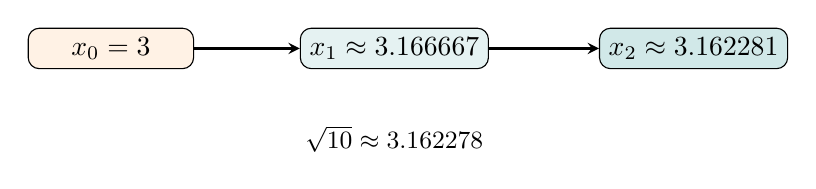
\begin{tikzpicture}[>=stealth,node distance=1cm]
\node[draw,rounded corners,fill=orange!10,minimum width=2.1cm] (a) at (0,0) {$x_0=3$};
\node[draw,rounded corners,fill=teal!10,minimum width=2.3cm] (b) at (3.6,0) {$x_1\approx3.166667$};
\node[draw,rounded corners,fill=teal!18,minimum width=2.3cm] (c) at (7.4,0) {$x_2\approx3.162281$};
\draw[->,thick] (a)--(b);\draw[->,thick] (b)--(c);
\node at (3.6,-1.15) {\small $\sqrt{10}\approx3.162278$};
\end{tikzpicture}

\end{center}
\medskip
\textbf{快记：}新点 $=$ 旧点 $-$“函数值 $\div$ 斜率”。\par\textbf{快懂：}用局部切线代替曲线，从切线横轴交点更新。\par\textbf{快用：}根号的迭代公式计算简便；只比较大小时优先直接平方。
\end{summarybox}
\clearpage
\begin{summarybox}
\textbf{\textcolor{CSummary}{和平方根估算的联系}}
\par\medskip
\begin{center}
% F087｜square 原创简明教学示意图
\begin{tikzpicture}[>=stealth,scale=.9]
\node[draw,fill=teal!8,rounded corners,minimum width=7.3cm,minimum height=1.5cm,align=center] at (4,0) {$x_{n+1}=\dfrac12\left(x_n+\dfrac{A}{x_n}\right)$};
\node at (4,-1.2) {\small 正数 $x_n$ 与 $A/x_n$ 的平均数};
\end{tikzpicture}

\end{center}
\medskip
F086 的近似 $t+(A-t^2)/(2t)$，正好就是 F087 对 $x^2-A=0$ 从 $x_0=t$ 出发的\textbf{第一次迭代}。两条结论角度不同：F086 主讲估值与误差，F087 主讲切线与重复更新。
\end{summarybox}
